\section{Físico-Química} \label{sec:fisquim}

Um dos métodos mais tradicionais em QSAR, a Análise Comparativa de Campo Molecular (CoMFA, do inglês \textit{Comparative Molecular Field Analysis}) \cite{Cramer1988}, consiste em otimizar a geometria da molécula de interesse e então colocá-la em uma caixa tridimensional, na qual uma sonda (como, por exemplo, um íon) percorrerá \( n \) pontos, sempre calculando as interações eletrostáticas e estéricas com a molécula. Esse procedimento é repetido para cada molécula do conjunto de \( m \) moléculas, gerando-se uma matriz \( A \in \mathbb{R}^{m \times n} \).

Define-se então um subespaço \( \mathcal{X} = C(A) = \text{span}\{A_1, A_2, \ldots, A_n\} \), em que \( C(A) \) é o espaço-coluna de \( A \) e \( A_i \) é a \( i \)-ésima coluna de \( A \). Posteriormente, partindo-se do entendimento que o subespaço \( \mathcal{X} \) também engloba ruídos e informações irrelevantes, gera-se uma nova base para um subespaço \( \mathcal{D} \subset \mathcal{X} \), com \( \dim(\mathcal{D}) < \dim(\mathcal{X}) \), aqui chamado de subespaço dos descritores selecionados, em alusão ao fato de que a hipótese central da QSAR é que esse subespaço é capaz de descrever satisfatoriamente o conjunto das moléculas.

\subsection{LQTA-QSAR}

Embora o formalismo proposto por \textcite{Hopfinger1997} tenha demonstrado bons resultados, sua metodologia de extração de descritores não contempla diretamente as interações eletrostáticas entre a molécula e o ambiente, limitando o realismo da modelagem. Visando superar essa limitação, \textcite{LQTAQSAR2009} propuseram, em 2009, o método LQTA-QSAR, que combina os princípios da CoMFA \cite{Cramer1988} com o formalismo 4D, incorporando descritores energéticos derivados do espaço conformacional da molécula.

No LQTA-QSAR, o Perfil de Amostragem Conformacional (CEP) da molécula é inserido em uma malha tridimensional. Cada ponto da malha é percorrido por uma sonda --- por exemplo, um íon \ce{NH3+} --- e, para cada posição, são calculadas as interações de Coulomb (\autoref{eq:coulomb}) e de Lennard-Jones (\autoref{eq:lj}) com todos os átomos do CEP. A \autoref{fig:LQTA-QSAR} ilustra esse processo para uma malha com resolução de 1 \AA.


\begin{figure}
    \centering
    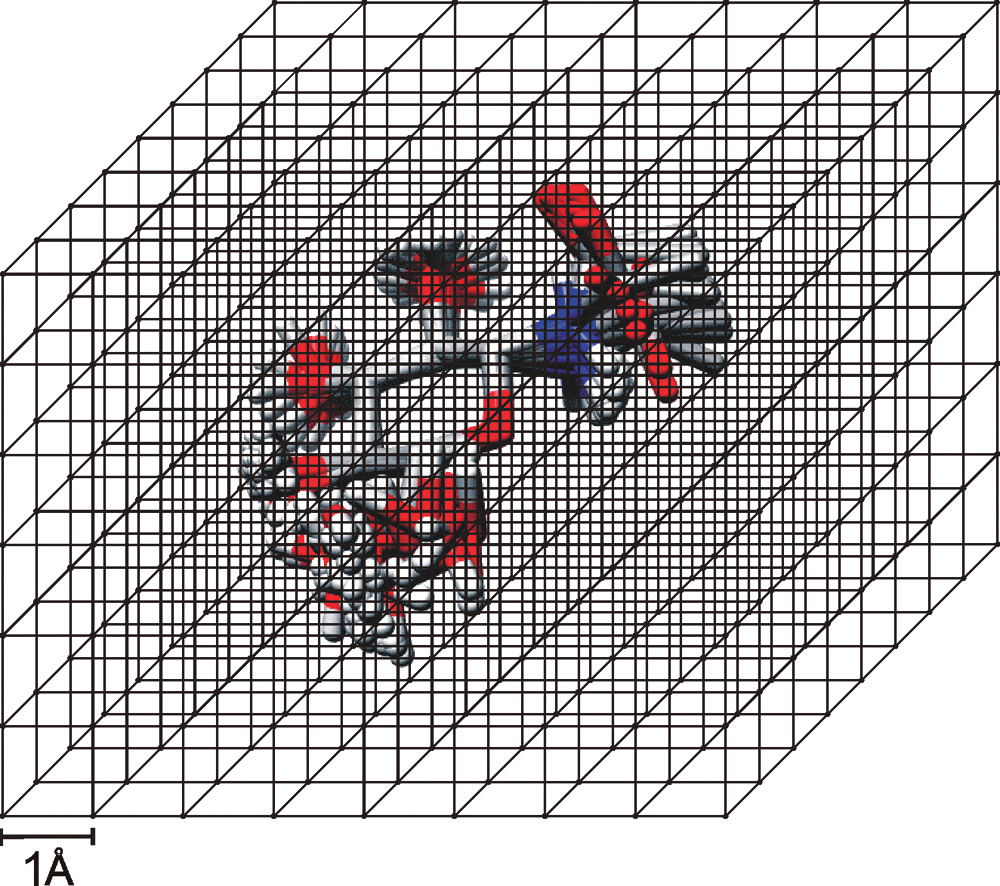
\includegraphics[width=0.5\textwidth]{img/LQTAQSAR_CEP.png}
    \caption{Exemplo de um perfil de amostragem conformacional (CEP) num grid do LQTA-QSAR de 1 \AA. Fonte: \textcite{LQTAQSAR2009}.}
    \label{fig:LQTA-QSAR}
  \end{figure}

Sejam $r_{ij}$ a distância entre o ponto $i$ da malha (onde está localizada a sonda) e o átomo $j$ do CEP; $\varepsilon$, a permissividade elétrica do meio; $n$, o número de conformações presentes no CEP; e $\{K_{ii}^{12}, K_{ii}^6, K_{jj}^{12}, K_{jj}^6\}$ os parâmetros do campo de força associados à sonda e aos átomos da molécula. As interações são dadas pelas expressões:

\begin{align}
    C &= \frac{1}{n} \sum_j \frac{q_i q_j}{4 \pi \varepsilon r_{ij}} \label{eq:coulomb} \\
    LJ &= \sum_j \left( \frac{K_{ij}^{12}}{r_{ij}^{12}} - \frac{K_{ij}^{6}}{r_{ij}^{6}} \right) \label{eq:lj} \\
    K_{ij}^{12} &= \sqrt{ \frac{K_{ii}^{12} \cdot K_{jj}^{12} }{n} } \\
    K_{ij}^{6} &= \sqrt{ \frac{K_{ii}^{6} \cdot K_{jj}^{6} }{n} }
\end{align}

Para cada CEP, gera-se um vetor de descritores $\vec{x}_i \in \RR^{2m}$, representando as energias calculadas nos pontos da malha. Considerando uma caixa cúbica de aresta $a$ e resolução de 1 \AA, são amostrados $a^3$ pontos, cada um com duas energias (Coulomb e Lennard-Jones), resultando em uma matriz de descritores $X \in \RR^{2a^3 \times m}$.

Apesar de eficiente, essa abordagem apresenta uma limitação importante: a malha pode conter pontos muito próximos aos átomos do CEP, fazendo $r_{ij} \to 0$. Nessas situações, \eqref{eq:coulomb} e \eqref{eq:lj} tendem ao infinito ($\lim_{r_{ij} \to 0} C = \lim_{r_{ij} \to 0} LJ = \infty$), produzindo valores de energia não realistas que comprometem a qualidade dos descritores e, consequentemente, a performance do modelo.

Em resumo, o LQTA-QSAR permite a amostragem do espaço conformacional de uma molécula por meio de uma malha tridimensional, associando a cada ponto vetores de energia obtidos a partir de interações físico-químicas simuladas com uma sonda. Esses vetores energéticos são então utilizados como descritores para a modelagem QSAR. Contudo, a presença de pontos com interações singularmente elevadas pode introduzir variáveis irrelevantes e comprometer a robustez estatística do modelo.

\subsection{LQTAGridHull — Amostragem Filtrada por Geometria Convexa}

Uma das principais limitações do LQTA-QSAR e de métodos relacionados, como o CoMFA, reside no fato de que a sonda pode ser posicionada muito próxima --- ou mesmo no interior --- de um átomo do CEP. Nessas condições, as interações de Coulomb e Lennard-Jones calculadas nos pontos da malha tendem ao infinito ($r_{ij} \to 0$), o que gera descritores fisicamente inverossímeis, reduz a robustez estatística dos modelos e compromete sua interpretabilidade.

Para mitigar esse problema, \textcite{Tenorio2018} propuseram o método \textit{LQTAGridHull}, que introduz o conceito de fecho convexo na etapa de amostragem dos descritores. Em geometria computacional, o \emph{fecho convexo} $\mathcal{F}(X)$ de um conjunto de pontos $X \subset \RR^d$ é definido como o menor conjunto convexo que o contém. Formalmente:

\begin{equation} \label{eq:def-convex-hull}
\mathcal{F}(X) = \left\{ \sum_{i=1}^{k} \lambda_i x_i \ \middle| \ x_i \in X, \lambda_i \ge 0, \sum_{i=1}^{k} \lambda_i = 1 \right\}
\end{equation}

A \autoref{fig:convex_hull_2d} ilustra esse conceito em duas dimensões, com os pontos de um conjunto $X \subset \RR^2$ (em azul) e seu fecho convexo $\mathcal{F}(X)$ (delineado pela linha vermelha).

\begin{figure}
  \centering
  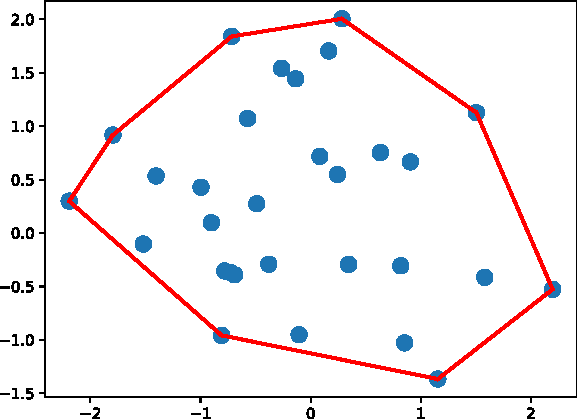
\includegraphics[width=0.5\textwidth]{img/convex_hull_2d.pdf}
  \caption{Exemplo de fecho convexo $\mathcal{F}(X)$ (linha vermelha) do conjunto $X \subset \RR^2$ (pontos azuis). Fonte: \textcite{Tenorio2018}.}
  \label{fig:convex_hull_2d}
\end{figure}

No contexto da 4D-QSAR, cada átomo de cada conformação no CEP é representado como um ponto $x_i \in X$, em que $X \subset \RR^3$. O fecho convexo tridimensional desses pontos, denotado por $\mathcal{H}(X)$, corresponde à menor região convexa que os contém, servindo como uma barreira natural para restringir a amostragem de descritores às regiões externas da densidade atômica.

A superfície $\partial \mathcal{H}(X)$ é então expandida radialmente por uma distância $r_0$, originando uma nova superfície $\mathcal{H}'(X)$:

\begin{equation}
\mathcal{H}'(X) = \left\{ x + r_0 \cdot \hat{n}_x \mid x \in \partial \mathcal{H}(X), \hat{n}_x \text{ é a normal externa em } x \right\}
\end{equation}

A partir dessa superfície inicial, define-se uma sequência de cascas esféricas com incrementos radiais $\Delta_r$:

\begin{equation}
\mathcal{H}^{(k)}(X) = \left\{ x + (r_0 + k \Delta_r) \cdot \hat{n}_x \right\}, \quad k = 0, \dots, l-1
\end{equation}

O número total de cascas, $l$, é dado por \eqref{eq:max-num-of-r-steps}. Em cada casca, define-se uma malha esférica com espaçamento angular $\Delta_\alpha$ em coordenadas esféricas $(\theta, \phi)$, resultando no número total de pontos amostrados, calculado em \eqref{eq:max-num-of-points}.

\begin{equation}
l = 1 + \left\lfloor \frac{r_{\mathrm{max}} - r_0}{\Delta_r} \right\rfloor
\label{eq:max-num-of-r-steps}
\end{equation}

\begin{equation}
Z = l \left[ \left\lfloor \frac{360}{\Delta_\alpha} \right\rfloor \cdot \left\lfloor \frac{180}{\Delta_\alpha} \right\rfloor - 2 \left( \left\lfloor \frac{180}{\Delta_\alpha} \right\rfloor - 1 \right) \right]
\label{eq:max-num-of-points}
\end{equation}

Para cada ponto $z_j$ da malha, as interações com os átomos do CEP são calculadas por:

\begin{align*}
d_j^{\text{C}} &= \sum_{i=1}^{N} \frac{q_i q_j}{4 \pi \varepsilon_0 \, \|z_j - x_i\|} \\
d_j^{\text{LJ}} &= \sum_{i=1}^{N} \left( \frac{A_{ij}}{\|z_j - x_i\|^{12}} - \frac{B_{ij}}{\|z_j - x_i\|^6} \right)
\end{align*}

